\documentclass[12pt]{beamer}
\usetheme[navbar=false, bkgimage=false, shadow=true]{Fermi}

\usepackage{graphicx}

\usepackage{amsmath}
\usepackage{xspace}
\usepackage{deluxetable}

\title{Search for Spatially Extended \textit{fermi}-LAT Sources Using Two Years of Flight
Data}
%\subtitle{\ldots}

\author{Joshua Lande}
\institute{SLAC/Stanford}
\email{joshualande@gmail.com}
\date{August 25, 2011}

\begin{document}

\section{Introduction}

The introduction goes here\ldots


Primary motivations for improved analysis
\begin{itemize}
  \item More data (3 years vs 18 months)
  \item Many new GeV pulsars
  \item Hope to find new PWN in the off-peak emission of \lat-detected \gev Pulsars.
  \item Going to higher energies thanks to improved IRFs.
  \item Better spatial/morphological analysis due to new \pointlike code.
\end{itemize}


\begin{frame}{Topics relevant to catalog}
  \begin{itemize}
        \item Monte Carlo study of false detection rate 
        \item LAT's detection threshold to extension
        \item Reanalysis of extended sources in 2FGL
        \item Testing AGN for extension
        \item (See presentation at Galactic splinter for rest of paper)
  \end{itemize}
\end{frame}

\begin{frame}{Fig. 3: Monte Carlo Study of false detection rate}
  \begin{columns}
    \column{.5\textwidth} 
    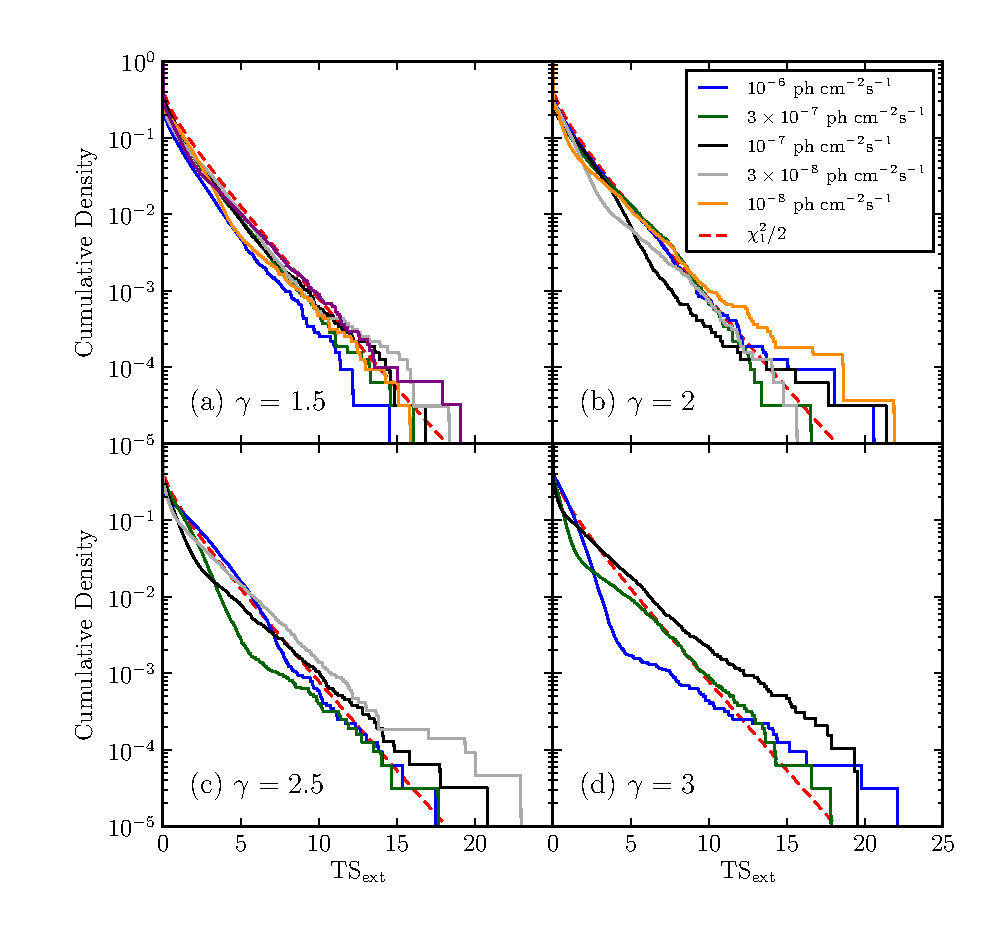
\includegraphics[scale=0.4]{../paper/mc_plots/ts_ext_emin_1000_color.eps}
    \column{.5\textwidth} 
    \begin{itemize}
      \item Simulate point sources
      \item One year simulation
      \item Against EGRET isotropic BG
      \item Vary flux, spectral index
      \item $\sim$30,000 sims per spectral model
      \item Test for extension
      \item Compare CDF of $\text{TS}_\text{ext}$ to $\chi^2_1/2$
      \item Good agreement with Wilks' Theorem
    \end{itemize}
  \end{columns}
\end{frame}

\begin{frame}{Fig. 4: Detection Threshold}
  \begin{columns}
    \column{.6\textwidth} 
    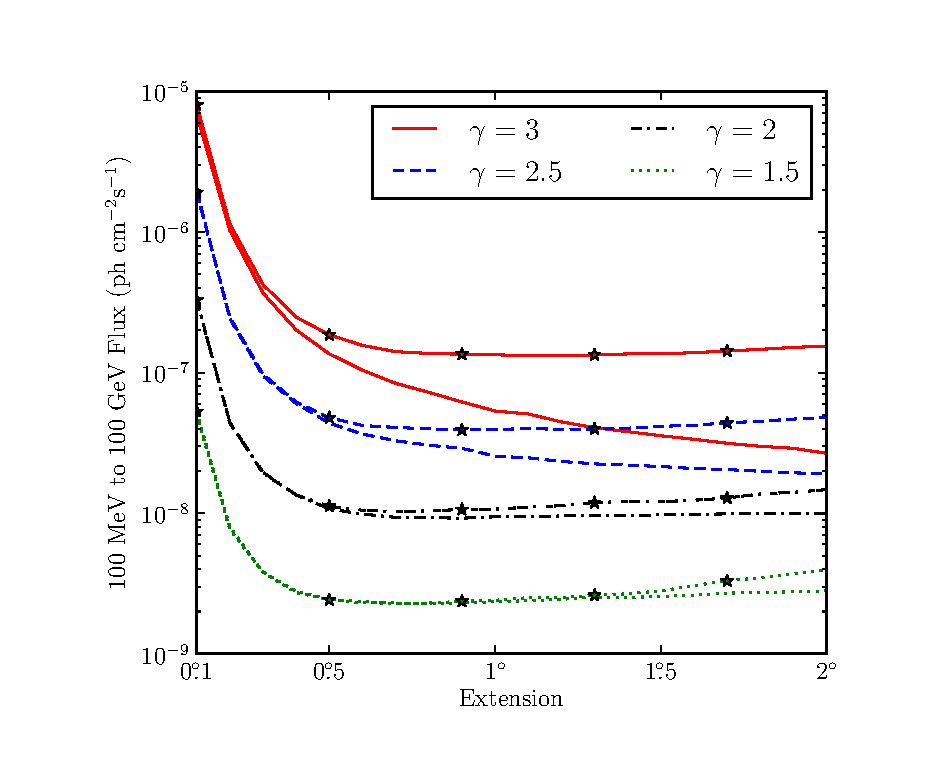
\includegraphics[scale=0.5]{../paper/mc_plots/index_sensitivity_color.eps}
    \column{.4\textwidth} 
    \begin{itemize}
      \item Detetion threshold to extension
      \item 2 years + isotropic bg
      \item Definition: $\langle\text{TS}_\text{ext}\rangle=16$
      \item Little sensitivity to small+soft sources
      \item Little improvement using 100 MeV to 1 GeV photons
    \end{itemize}
  \end{columns}
\end{frame}

\begin{frame}{Fig. 5: Threshold vs background}
  \begin{columns}
    \column{.6\textwidth} 
    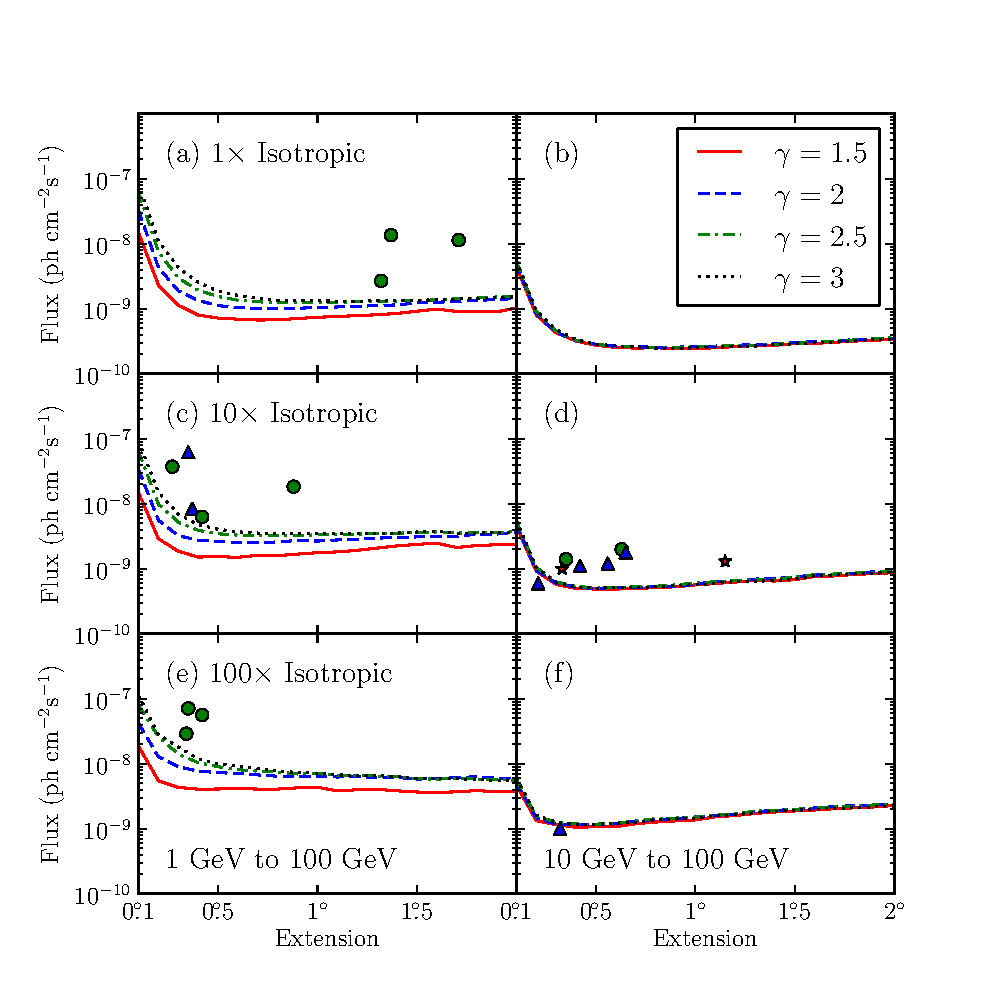
\includegraphics[scale=0.5]{../paper/mc_plots/all_sensitivity_color.eps}
    \column{.4\textwidth} 
    \begin{itemize}
      \item Vary 
        \begin{itemize}
          \item spectral index, 
          \item diffuse normalization
          \item energy range
        \end{itemize}
      \item Overlay extended sources
      \item Reference for future publications
    \end{itemize}
  \end{columns}
\end{frame}

\begin{frame}{Fig. 6: Threshold vs time}
  \begin{columns}
    \column{.6\textwidth} 
    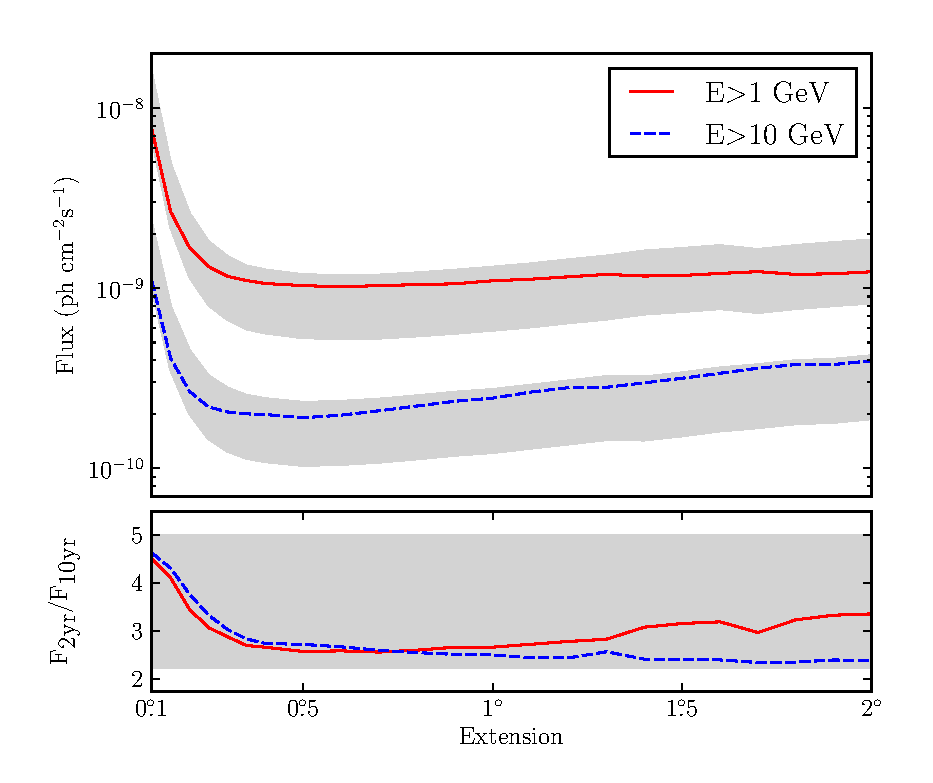
\includegraphics[scale=0.5]{../paper/mc_plots/time_sensitivity_color.eps}
    \column{.4\textwidth} 
    \begin{itemize}
      \item Calculate 10 year detection
        threshold
        \begin{itemize}
          \item With MC simulationn
          \item Projected from 2 years by $\sqrt{\text{time}}$ and 
            time
        \end{itemize}
      \item Sensitivity $>\sqrt{\text{time}}$ for
        small extended sources
    \end{itemize}
  \end{columns}
\end{frame}


\begin{frame}{Fig. 6: $\text{TS}_\text{ext}$ for 2LAC AGN}

  \begin{columns}
    \column{.6\textwidth} 
    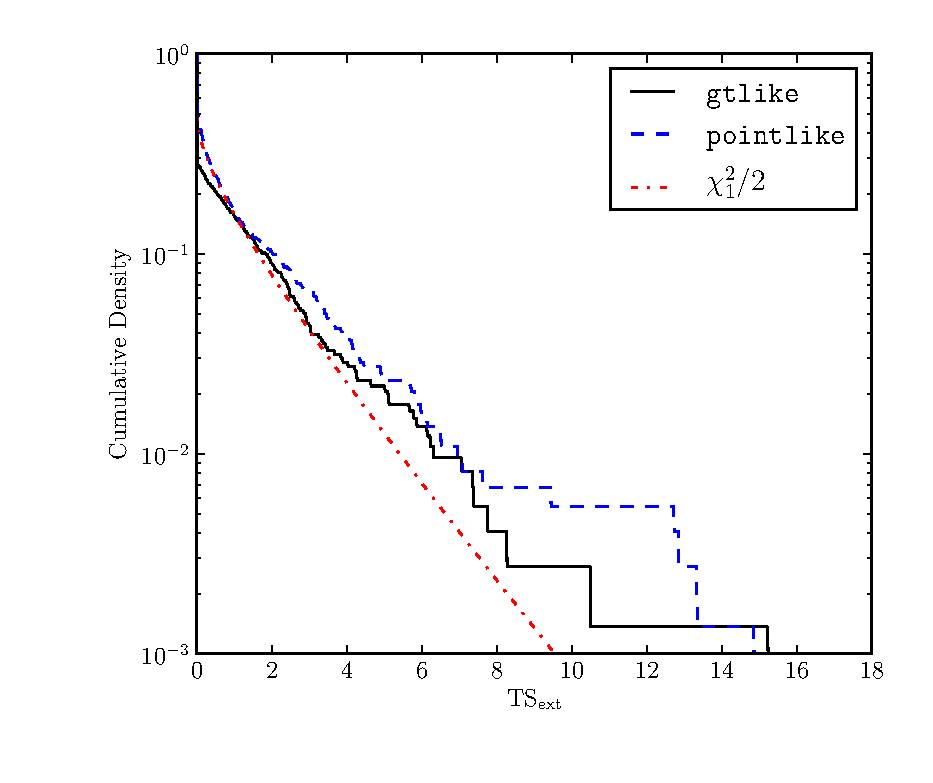
\includegraphics[scale=0.5]{../paper/source_plots/agn_color.eps}
    \column{.4\textwidth} 
    \begin{itemize}
      \item 885 clean AGN in 2LAC
        \item Test 783 of these (with $\text{TS}>25$)
        for extension
      \item Compare CDF of $\text{TS}_\text{ext}$ to $\chi^2_1/2$
      \item Don't find AGN to be extended
    \end{itemize}
  \end{columns}
\end{frame}

\begin{frame}{Table. 3: Reanalyze 12 sources in 2FGL}
    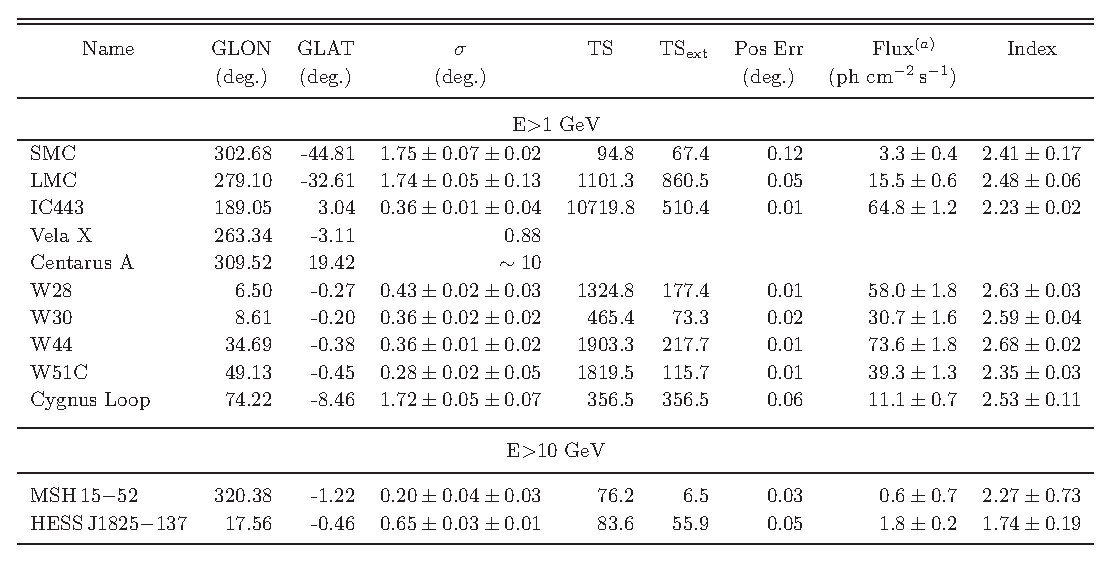
\includegraphics[scale=0.5]{tables/table3.eps}
  \begin{itemize}
    \item Test 12 2FGL sources for extension
    \item Assume radially symmetric disk spatial model
    \item Improved models could be included in future catalog
  \end{itemize}
\end{frame}

\begin{frame}{Table. 4: 9 more extended sources}
    \includegraphics[scale=0.45]{tables/table4.eps}

    Extended sources could be included in future catalog
\end{frame}


\end{document}
